\documentclass[10pt,journal]{IEEEtran}
\usepackage[T1]{fontenc}
\usepackage{lmodern}
\usepackage{microtype}
\usepackage{cite}
\usepackage{amsmath,amssymb}
\usepackage{graphicx}
\usepackage{booktabs}
\usepackage{algorithm}
\usepackage{algpseudocode}
\usepackage{url}
\usepackage{balance}
\usepackage[hidelinks]{hyperref}

\begin{document}
\title{Polarity-Aware Logic Optimization with\\Mixed Majority-Minority Inverter Graphs}
\author{Mrunal~Shende%
\thanks{M.~Shende is with the Department of Computer Science and Engineering,
Indian Institute of Technology Indore, Madhya Pradesh, India 453552.
E-mail: mrunalshende05@gmail.com.}}
\markboth{IEEE Embedded Systems Letters}{}
\maketitle

\begin{abstract}
Majority-inverter graphs (MIGs) encode signal polarity on complemented edges.
Explicit minority (MIN) nodes preserve Boolean expressiveness but change the
optimization representation. We evaluate a two-stage native MAJ/MIN flow
against a pure-MIG flow with comparable generic structural optimization from
the same starting networks. Across twelve EPFL circuits, both flows pass raw
ABC combinational equivalence checking against the original functions. The
mMIG flow reduces aggregate MAJ+MIN nodes by 0.89\% (15,205 to 15,070) and
nonconstant complemented graph connections by 7.38\% (6,501 to 6,021); the
latter improve on eleven circuits and tie on one. A round-capped pure-MIG
search retains a 7.43\% edge gap, although two circuits do not reach the mMIG
runtime. Direct MIN lowering followed by pure-MIG phase optimization yields
6,668 complemented connections, 2.57\% more than the matched pure MIG. The
measured reduction is specific to the native mixed representation and does
not establish mapped area or inverter-cell savings.
\end{abstract}
\begin{IEEEkeywords}
logic synthesis, majority-inverter graphs, minority gates, polarity optimization
\end{IEEEkeywords}
\IEEEpeerreviewmaketitle

\section{Introduction}
\label{sec:intro}
Majority-inverter graphs (MIGs) represent combinational logic with
three-input majority nodes and complemented edges~\cite{amaru2016mig}.
The complement bit on a connection records signal polarity. Pure-MIG
polarity optimization can move these bits without changing the graph
topology~\cite{testa2016inv}. A mixed majority-minority inverter graph
(mMIG) additionally labels nodes as minority (MIN). Because MIN is the
complement of MAJ, this changes neither Boolean expressiveness nor the
number of inputs to a node. It does change the available native polarity
assignments and mixed-graph rewrite choices~\cite{aalam2021mmig}.

The question addressed here is whether a native MAJ/MIN flow finds a
different structural outcome than a pure-MIG flow that also performs
structural optimization. A comparison with only fixed-topology phase
optimization cannot separate the value of the mixed representation from
generic rewriting and resubstitution effort. We therefore run both flows
from the same archived MIG for each circuit and report logic nodes and
complemented graph connections separately.

This letter contributes (i) a two-stage mMIG flow combining mixed structural
optimization with fixed-topology phase reassignment, (ii) a matched
pure-MIG structural and phase control, and (iii) twelve-circuit results
including raw equivalence checks, direct MIN lowering, and a pure-MIG
time-budget sensitivity test.\footnote{Source and reproducibility artifact:
\url{https://github.com/Mrunal321/mmig-polarity-optimization}, release
v1.1-esl-revision.} The mMIG flow has 0.89\% fewer aggregate
logic nodes and 7.38\% fewer native complemented connections than the
matched control, while taking about ten times longer. These data describe
the tested structural representations; they do not isolate MIN from every
other implementation difference.

\section{Mixed MAJ/MIN Representation}
\label{sec:representation}
For Boolean inputs $a,b,c$, the node functions are
\begin{equation}
\begin{aligned}
\mathrm{MAJ}(a,b,c)&=ab+ac+bc,\\
\mathrm{MIN}(a,b,c)&=\overline{\mathrm{MAJ}(a,b,c)}.
\end{aligned}
\label{eq:gates}
\end{equation}
An mMIG is a directed acyclic graph with MAJ or MIN internal nodes
and regular or complemented connections. A MIN node can be represented
by MAJ plus output complementation, so a mixed graph does not add Boolean
functions. It makes that polarity an explicit node choice, which permits
local gate-type and edge-phase changes during optimization.

We report $G=N_{\mathrm{MAJ}}+N_{\mathrm{MIN}}$ and $I$, the number of
complemented connections whose source is nonconstant. $I$ includes
gate-input and primary-output connections but excludes connections from
the constant node. Depth $D$ is the maximum logic-node level. LUT6 count
and LUT depth are secondary mapping diagnostics. $I$ is a structural graph
metric and is not a physical inverter-cell count.
We count each graph connection separately, including multiple fanouts
from one source; no fanout-dependent cell or wire cost is inferred.
Reporting $G$ and $I$ as separate objectives avoids choosing a
technology-dependent exchange rate between a logic node and a complement.

\section{Two-Stage mMIG Optimization}
\label{sec:method}
The mixed flow builds on existing \textsc{mockturtle} rewriting,
resubstitution, cut rewriting, and refactoring machinery
\cite{soeken2022libraries,riener2019generic}. Stage~1 seeds MIN
polarities, runs mixed algebraic and polarity operations, applies bounded
window resynthesis, and executes two advanced \texttt{compress2rs} rounds.
The round objective orders gate count before native complemented-edge count;
depth may increase. Balancing is disabled. Candidate passes are guarded by
internal equivalence checks. Minority seeding, cone polarity changes, and
mixed phase choices are specific to the extended representation; generic
rewriting and resubstitution primitives are not new algorithms here.
The internal advanced-round guard uses the raw native complement count,
including constant-source connections, whereas the reported $I$ excludes
them. A gate reduction may be accepted with more raw complements within
the configured allowance. This distinction matters when interpreting
intermediate passes: the paper reports the final nonconstant count, not
the optimizer's internal acceptance score.

Stage~1 writes a BLIF that Stage~2 reimports. This boundary preserves the
audited gate-incidence topology but does not preserve explicit MIN labels:
all imported gates initially have MAJ labels. Stage~2 applies mixed-phase
and two-phase optimization, allowing MAJ/MIN relabeling and input/output
phase reassignment without changing that topology. The final native MIN
counts therefore arise from Stage~2, not from direct carry-through of
Stage~1 type labels. The topology audit finds unchanged gate count, depth,
and incidence for all twelve circuits. Algorithm~\ref{alg:flow} summarizes
the executed sequence.
The reimport makes the second stage a phase search on the Stage~1
topology rather than a continuation of its in-memory MIN labels. This
implementation detail is necessary to reproduce the archived outputs.

\begin{algorithm}[t]
\caption{Two-stage native mMIG optimization}
\label{alg:flow}
\begin{algorithmic}[1]
\Require Starting MIG $N$; reference function $F$
\Ensure Equivalent mixed network $N^{*}$
\State $X\gets\mathrm{ImportMixed}(N)$
\State $X\gets\mathrm{SeedMinority}(X)$
\State $X\gets\mathrm{GuardedRewriteAndPolarity}(X)$
\State $X\gets\mathrm{GuardedWindowResynthesis}(X)$
\For{$r=1,2$}
  \State $X\gets\mathrm{GuardedCompress2rsRound}(X)$
\EndFor
\State $Y\gets\mathrm{ReimportBLIF}(X)$ \Comment{MIN labels lost}
\State $Y\gets\mathrm{MixedPhase}(Y)$
\State $N^{*}\gets\mathrm{TwoPhase}(Y)$ \Comment{topology fixed}
\State \textbf{assert} $\mathrm{ABC\_CEC}(F,N^{*})$
\State \Return $N^{*}$
\end{algorithmic}
\end{algorithm}

The frozen Stage~1 uses three algebraic iterations, four-input window
cuts, at most eight internal window nodes, 2,048 expressions, eight
matches per root, and 128 roots. It enables don't-care and zero-gain
operations. Exact commands and the hashed binary are in the companion
artifact. The second stage only changes phases and node types.
The source uses miter-based equivalence guards around the mixed
structural passes and checks selected resubstitution candidates. Final
raw ABC CEC is an independent verification step against the original
benchmark function, not the criterion used to rank candidate graphs.

\section{Experimental Evaluation}
\label{sec:eval}
\subsection{Setup and controls}
We evaluate twelve EPFL combinational benchmarks~\cite{epfl2015}.
For each benchmark, three fixed flows use the \emph{same} archived starting
MIG: $T$ is our local Testa-style fixed-topology pure-MIG polarity control;
$P$ is a pure-MIG structural-plus-phase control; and $M$ is the frozen
two-stage \texttt{zg2} mMIG flow. $P$ uses a generic standard pre-pass,
two \texttt{compress2rs} rounds, and a pure-MIG phase pass. It matches
the broad structural opportunities of $M$, including rewriting,
resubstitution, cut rewriting, and refactoring, but their libraries,
candidate limits, and internal CEC schedules are not identical. Thus
$M-P$ is the primary fixed-flow comparison, not a same-runtime or
single-feature MIN ablation.
Both $P$ and $M$ use area mode, two compress-style rounds, zero-gain
moves, a four-input cut setting where available, and a final phase
optimization. $P$ receives an additional generic standard pre-pass.
The mixed flow alone has minority seeding, cone polarity changes, and
its bounded mixed window search. The underlying rewrite libraries and
phase search spaces differ, so the comparison controls starting point
and broad optimization opportunity, not every primitive operation.

All twelve starting MIGs and all 36 final $T/P/M$ outputs passed direct
raw ABC CEC against their original EPFL BLIFs. Each output was mapped by
the same ABC script, \texttt{strash; if -K 6 -a}. The $M$ profile was
developed with knowledge of these twelve benchmarks; the starting MIG
choice was also informed by earlier mMIG-score selection. These rows
are development-set results, not a holdout generalization study. $T$
is a local implementation of Testa-style transformations, not the
released program of Testa \emph{et al.}~\cite{testa2016inv}.
The archived starting networks were selected before this control
study using earlier mixed-flow results. All three flows share each
selected input, but this choice can favor $M$ at the dataset level.
We therefore report a fixed-profile observation on the twelve circuits,
without claiming an unbiased sample of starting MIGs.

% AUTO-GENERATED -- DO NOT EDIT
\begin{table*}[t]
\caption{Matched structural results. $P$ is the pure-MIG control and $M$ is the frozen mMIG flow. $G$ counts MAJ+MIN nodes; $I$ counts complemented nonconstant graph connections. Negative changes favor $M$.}
\label{tab:primary}
\centering
\begin{tabular}{lrrrrrrr}
\toprule
Circuit & $P:G$ & $M:G$ & $\Delta G$ (\%) & $P:I$ & $M:I$ & $\Delta I$ (\%) & MIN \\
\midrule
adder & 384 & 384 & 0.00 & 255 & 255 & 0.00 & 0 \\
arbiter & 3632 & 3597 & -0.96 & 1026 & 987 & -3.80 & 205 \\
bar & 2460 & 2464 & +0.16 & 675 & 624 & -7.56 & 45 \\
cavlc & 527 & 524 & -0.57 & 243 & 180 & -25.93 & 57 \\
ctrl & 65 & 64 & -1.54 & 29 & 27 & -6.90 & 1 \\
dec & 304 & 304 & 0.00 & 16 & 8 & -50.00 & 4 \\
i2c & 848 & 842 & -0.71 & 401 & 282 & -29.68 & 129 \\
int2float & 169 & 167 & -1.18 & 79 & 54 & -31.65 & 25 \\
max & 2093 & 2052 & -1.96 & 1102 & 1013 & -8.08 & 70 \\
priority & 369 & 356 & -3.52 & 150 & 129 & -14.00 & 14 \\
router & 136 & 134 & -1.47 & 43 & 37 & -13.95 & 10 \\
voter & 4218 & 4182 & -0.85 & 2482 & 2425 & -2.30 & 56 \\
\midrule
Sum & 15205 & 15070 & -0.89 & 6501 & 6021 & -7.38 & --- \\
\bottomrule
\end{tabular}
\end{table*}


\subsection{Matched pure-MIG comparison}
Table~\ref{tab:primary} reports the native structural results. Relative
to $P$, $M$ changes aggregate $G$ from 15,205 to 15,070 ($-0.89\%$)
and $I$ from 6,501 to 6,021 ($-7.38\%$). Complemented connections
fall on eleven circuits and tie on \texttt{adder}; gate count falls on
nine, ties on two, and rises on \texttt{bar}. Fig.~\ref{fig:edges}
shows the edge changes without removing the tie. Relative to $T$, $M$
has 2.48\% fewer gates and 10.79\% fewer native complemented connections,
but the matched $P$ flow itself improves on $T$ by 1.61\% and 3.67\%,
respectively. Table~\ref{tab:primary} lists $T$'s edge count per circuit;
its fixed-topology pass leaves gate count unchanged. $M$ uses fewer edges
than $T$ on ten circuits, ties on \texttt{adder}, and is worse on
\texttt{bar} (624 versus 486). The $T$ comparison alone would overstate
the mixed-flow advantage attributable to representation. Published
Testa numbers use different starting MIGs and cannot be inserted as
same-input results~\cite{testa2016inv}.
The largest percentage change is \texttt{dec} ($16$ to $8$ edges), where
the denominator is small. On the much larger \texttt{voter}, the
corresponding change is $2{,}482$ to $2{,}425$ edges ($-2.30\%$).
The aggregate reduction sums actual connections across the circuit set;
it is not the mean of per-circuit percentages. On \texttt{bar}, $M$
uses four more logic nodes but 51 fewer complemented connections than
$P$. These circuit-level differences remain visible in Table~\ref{tab:primary}.

\begin{figure}[t]
\centering
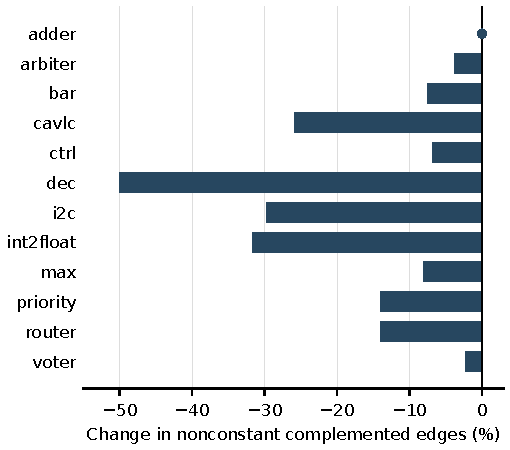
\includegraphics[width=\columnwidth]{figures/m_vs_p_edges.pdf}
\caption{Change in nonconstant complemented connections for $M$ versus $P$.
Negative values favor the mixed graph; \texttt{adder} ties.}
\label{fig:edges}
\end{figure}

% AUTO-GENERATED -- DO NOT EDIT
\begin{table}[t]
\caption{Aggregate context for the three fixed flows.}
\label{tab:summary}
\centering
\begin{tabular}{lrrrr}
\toprule
Flow & $G$ & $I$ & LUT6 & Time (s) \\
\midrule
T & 15454 & 6749 & 5863 & 0.33 \\
P & 15205 & 6501 & 5815 & 24.08 \\
M & 15070 & 6021 & 5867 & 239.87 \\
\bottomrule
\end{tabular}
\end{table}


Table~\ref{tab:summary} gives mapping and runtime context. $P$ maps
to 5,815 LUT6s and $M$ to 5,867 under the common mapper. The structural
polarity reduction does not produce an aggregate LUT6 reduction. $M$
also takes 239.87~s versus 24.08~s for $P$. The area-oriented flow
does not enforce depth non-regression: $M$ is deeper on three circuits,
equal on six, and shallower on three; per-circuit depths and LUT depths
remain in the artifact.
The LUT6 result is a structural mapping diagnostic. It is not an
estimate of standard-cell area or of the cost of realizing MIN in a
specific technology. The common mapper can absorb phases and restructure
logic, so it need not preserve the ordering of native graph-edge counts.

\subsection{Representation and runtime controls}
To test the role of explicit MIN labels, we directly expand the final
native MIN nodes into MAJ plus required phases and then apply the same
pure-MIG phase optimization. The resulting MAJ-only networks have 6,668
nonconstant complemented connections, versus 6,021 natively and 6,501
for $P$. The lowered result is 2.57\% \emph{higher} than $P$; every
lowered output passes raw ABC CEC. The reduction is specific to the
native MAJ/MIN representation and does not establish a superior
MAJ/INV-only realization.
Raw lowering before the pure-MIG phase pass has 7,028 connections; the
phase pass removes 360, but does not reach $P$'s 6,501. Gate count,
depth, and incidence topology are unchanged by the direct lowering
and phase experiment. This ablation isolates representation of the
final $M$ graph; it does not prove which Stage~1 pass caused the
topology chosen by the mixed flow.
% AUTO-GENERATED -- DO NOT EDIT
\begin{table}[t]
\caption{Direct MIN-lowering ablation across twelve circuits. The three $M$ rows share gate-incidence topology.}
\label{tab:lowering}
\centering
\begin{tabular}{lrrr}
\toprule
Representation & $G$ & $I$ & MIN \\
\midrule
$M$ native & 15070 & 6021 & 616 \\
$M$ MAJ-only raw & 15070 & 7028 & 0 \\
$M$ MAJ-only + phase & 15070 & 6668 & 0 \\
$P$ pure MIG & 15205 & 6501 & 0 \\
\bottomrule
\end{tabular}
\end{table}


A separate pure-MIG search extends $P$ within an approximate per-circuit
$M$ time budget, subject to a 20-round cap. It reaches 15,136 gates,
6,504 complemented connections, and 5,829 LUT6s. Against this control,
$M$ has 0.44\% fewer gates and 7.43\% fewer native complemented
connections. Ten circuits reach or slightly exceed their time target;
\texttt{max} and \texttt{voter} stop at the round cap first. This is a
sensitivity check, not an equal-runtime result.
In particular, the capped $P$ search uses 28.18~s against the
72.35~s $M$ target on \texttt{max}, and 50.13~s against 86.55~s on
\texttt{voter}. Allowing more pure-MIG rounds could change the
comparison. Conversely, reducing $M$'s search or equivalence-checking
effort might change its result. The primary table holds each flow
at its frozen profile and makes no equal-work attribution.

\subsection{Scope of the structural result}
The three controls answer different questions. $T$ asks how far a local
pure-MIG phase pass moves complements without modifying topology. $P$
asks what additional generic pure-MIG structure search provides from
that same starting point. $M$ asks what the frozen mixed flow produces
after both structural and phase stages. Their common inputs and CEC
checks make the output metrics directly comparable, but the flows
do not execute the same candidate sequence. In particular, $P$ has
no operation identical to the mixed minority-seeding and node-type
phase choices, while its generic local libraries are not the same as
the mixed implementations. The $M-P$ difference therefore cannot
be assigned solely to explicit MIN nodes.

The native-to-lowered comparison provides a narrower representation
test. Each lowered circuit preserves the final mixed graph's incidence
topology and logic-node count, changing only the representation of
MIN and then the allowed pure-MIG phases. Its 647 additional
nonconstant complemented connections after pure-MIG phase optimization
show that the native MIN labels carry a measurable edge-count benefit
for these selected topologies. This benefit says nothing about the
cost of a physical MIN implementation. It also does not show that the
mixed structural passes would beat a pure-MIG topology search given
identical runtime and candidate opportunities.

The twelve benchmarks were used during profile development, and the
one chosen starting MIG per benchmark was selected from earlier
experiments. We report exact outcomes for those selected cases, not
an estimate of expected improvement on unseen circuits. No
standard-cell mapping, device model, or post-layout analysis is used
to translate $I$ into circuit area or energy. Future evaluation must
hold the search budget and target technology fixed before making
either claim.

\balance
\section{Related Work}
\label{sec:related}
MIG algebra and Boolean optimization were established by Amar\`u
\emph{et al.}~\cite{amaru2016mig}. Testa \emph{et al.} studied
fixed-topology inversion optimization in pure MIGs~\cite{testa2016inv}.
Generic rewriting, resubstitution, and refactoring flows provide the
structural machinery used by both controls~\cite{riener2019generic}.
Aalam \emph{et al.} introduced mMIG synthesis and inversion
optimization~\cite{aalam2021mmig}; our earlier mMIG work studied
additional algebra and circuit metrics~\cite{shende2025mmig}. This
letter focuses on the matched pure-MIG control and direct native-MIN
lowering needed to interpret the structural result.

\section{Conclusion}
\label{sec:conclusion}
Across twelve CEC-verified EPFL circuits, the frozen mixed flow uses
0.89\% fewer MAJ+MIN nodes and 7.38\% fewer nonconstant complemented
graph connections than a matched pure-MIG structural and phase flow.
The native edge advantage disappears after direct MIN lowering, while
the mixed flow takes about ten times longer and maps to slightly more
LUT6s. These results support a representation-specific structural
polarity reduction under the tested profiles. They do not show mapped
inverter, area, energy, or equal-runtime improvement.

\bibliographystyle{IEEEtran}
\bibliography{refs}
\end{document}
